	\documentclass[14pt]{extreport}
\usepackage{extsizes}
	\usepackage[frenchb]{babel}
	\usepackage[utf8]{inputenc}  
	\usepackage[T1]{fontenc}
	\usepackage{amssymb}
	\usepackage[mathscr]{euscript}
	\usepackage{stmaryrd}
	\usepackage{amsmath}
	\usepackage{tikz}
	\usepackage[all,cmtip]{xy}
	\usepackage{amsthm}
	\usepackage{varioref}
	\usepackage[ margin=1in]{geometry}
	\geometry{a4paper}
	\usepackage{lmodern}
	\usepackage{hyperref}
	\usepackage{array}
	\usepackage{float}
	\usepackage{easytable}
	 \usepackage{fancyhdr}\usepackage{longtable}
	 \usetikzlibrary{shapes.misc}

\tikzset{cross/.style={cross out, draw=black, minimum size=2*(#1-\pgflinewidth), inner sep=0pt, outer sep=0pt},
%default radius will be 1pt. 
cross/.default={1pt}}

	\pagestyle{fancy}
	\theoremstyle{plain}
	\fancyfoot[C]{\empty} 
	\fancyhead[L]{Interrogation}
	\fancyhead[R]{10 mai 2023}
	
	
	\title{Contrôle chapitre 7}
	\date{}
	\begin{document}

\begin{center}{\Large Contrôle chapitre 7}\end{center}



\textbf{Exercice 1}  % 4 points

Pour chacune des propositions suivantes, la traduire par une expression littérale : 

\begin{enumerate}
\item La somme de $a$ et de $b$
\item Le produit de $3$ par $x$
\item La différence entre $a$ et le produit de $4$ par $b$
\item La somme du produit de $3$ par $c$ et du quotient de $4$ par $b$. 
\end{enumerate}


\textbf{Exercice 2} % 1 / 1.5 / 1.5  -> 4 points

Évaluer les expressions suivantes aux valeurs indiquées : 

\begin{enumerate}
\item $3\times a - 5$ en $a=1$, 

\item $a + 2 \times 3$ en $a= -4$, 
\item $a + a \times a$ en $a= 3$, 
\item $ a \times b - (a - 1) \times b $ en $a= 9$ et $b= 12$. 
\end{enumerate}

 \textbf{Exercice 3 }
 
On achète $7$ cahiers et $3$ classeurs.

\begin{enumerate}
\item En notant $x$ le prix d'un cahier, et $y$ celui d'un classeur, écrire une expression littérale donnant le coût total de cet achat. 
\item Si un cahier coûte $2,10$ euros, et un classeur $2,9$ euros, combien a-t-on dépensé ? 
\item On suppose que l'on a dépensé $27$ euros et $80$ centimes au total. Est-il possible qu'un cahier coûte $2,90$ euros et un cahier $2,50$ euros ? 
\item On suppose que l'on a dépensé au total $21,90$ euros, et on se souvient qu'un cahier coûte $2,10$ euros. Retrouver le prix d'un classeur. 
\end{enumerate}
 
\textbf{Exercice 4} % 6 points

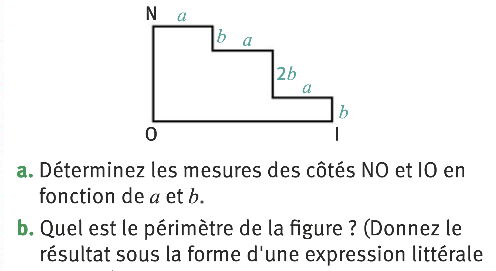
\includegraphics[scale=1.4]{exo}

\newpage
\begin{center}{\Large Contrôle chapitre 7}\end{center}
\textbf{Exercice 1}  % 4 points

Pour chacune des propositions suivantes, la traduire par une expression littérale : 

\begin{enumerate}
\item La somme de $d$ et de $a$
\item Le produit de $x$ par $4$
\item La différence entre $a$ et le produit de $4$ par $b$
\item La somme du produit de $3$ par $c$ et du quotient de $4$ par $b$. 
\end{enumerate}


\textbf{Exercice 2} % 1 / 1.5 / 1.5  -> 4 points

Évaluer les expressions suivantes aux valeurs indiquées : 

\begin{enumerate}
\item $3\times a - 5$ en $a=2$, 

\item $a + 2 \times 3$ en $a= -3$, 
\item $a + a \times a$ en $a= 3$, 
\item $ a \times b - (a - 1) \times b $ en $a= 9$ et $b= 12$. 
\end{enumerate}

 \textbf{Exercice 3 }
 
On achète $7$ cahiers et $3$ classeurs.

\begin{enumerate}
\item En notant $x$ le prix d'un cahier, et $y$ celui d'un classeur, écrire une expression littérale donnant le coût total de cet achat. 
\item Si un cahier coûte $2,10$ euros, et un classeur $2,9$ euros, combien a-t-on dépensé ? 
\item On suppose que l'on a dépensé $27$ euros et $80$ centimes au total. Est-il possible qu'un cahier coûte $2,90$ euros et un cahier $2,50$ euros ? 
\item On suppose que l'on a dépensé au total $21,90$ euros, et on se souvient qu'un cahier coûte $2,10$ euros. Retrouver le prix d'un classeur. 
\end{enumerate}
 
\textbf{Exercice 4} % 6 points

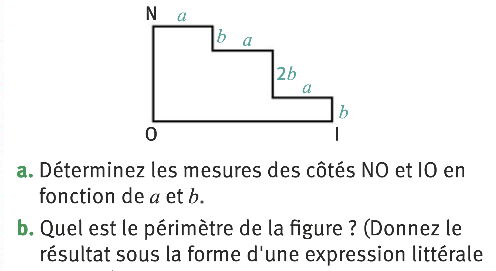
\includegraphics[scale=1.4]{exo}
 
 
 
 
 
 
 \end{document}